\documentclass{article}

\usepackage[margin=2.5cm]{geometry}

\usepackage[spanish]{babel}
\usepackage[T1]{fontenc}

\usepackage{graphicx}
\usepackage{fancyhdr}
\usepackage{fancyvrb}

\usepackage{tcolorbox}

\usepackage{listings}
\usepackage{xcolor}

\definecolor{codegreen}{rgb}{.2,0.6,0}
\definecolor{codegray}{rgb}{0.5,0.5,0.5}
\definecolor{codepurple}{rgb}{0.58,0,0.82}
\definecolor{codeblue}{rgb}{0,0.4,0.82}
\definecolor{codeorange}{rgb}{0.94,0.34,0.0}
\definecolor{backcolour}{rgb}{0.95,0.95,0.92}
\definecolor{backcolourgray}{rgb}{0.92,0.92,0.92}
\definecolor{codewhite}{rgb}{1,1,1}

\lstdefinestyle{mystyle}{
    backgroundcolor=\color{backcolourgray},   
    commentstyle=\color{codegreen},
    keywordstyle=\color{codeblue},
    numberstyle=\tiny\color{black},
    stringstyle=\color{codeorange},
    basicstyle=\ttfamily\footnotesize,
    breakatwhitespace=false,         
    breaklines=true,                 
    captionpos=b,                    
    keepspaces=true,                 
    %numbers=left,                    
    numbersep=5pt,                  
    showspaces=false,                
    showstringspaces=false,
    showtabs=false,                  
    tabsize=2,
    extendedchars=true,
    frame=single
    %, basicstyle=\footnotesize
}
\lstset{style=mystyle}

\usepackage{hyperref}
\hypersetup{
    colorlinks=true,
    linkcolor=blue,
    filecolor=magenta,      
    urlcolor=cyan,
}

\pagestyle{fancy}
\fancyhf{}
\rhead{Sistemas Operativos. Práctica 3.}
\lhead{Pablo Cuesta Sierra y Álvaro Zamanillo Sáez}
\cfoot{\thepage}



\setlength{\parskip}{0.15cm}



\begin{document}

\title{Sistemas Operativos. Práctica 3.}
\author{Pablo Cuesta Sierra y Álvaro Zamanillo Sáez}
\date{}
\maketitle

\begin{tcolorbox}
\tableofcontents
\end{tcolorbox}

\pagebreak

\addcontentsline{toc}{section}{Calificación base}
\section*{Calificación base}

\addcontentsline{toc}{subsection}{Nivel 1: Minero multihilo}
\subsection*{Nivel 1: Minero multihilo}

    Para este primer nivel hemos diferenciado dos partes. En primer lugar iniciar correctamente los segmentos de memoria compartida del bloque y la red, y por otro lado, la creación de los hilos y su correcta terminanción. 

    En la red, hemos incluido más atributos (para siguientes niveles) y es el primer minero el que se encarga de inicializarlos correctamente.
    De la misma forma, si el minero crea el segmento que corresponde al bloque, configura una "primera solución" que se usará para generar el primer \textit{target} (y por ende, el resto).

    Por otro lado, para lo relativo a los hilos, alocamos un \textit{array} de \textbf{pthread\_t} e iniciamos la estructura de minado que cada trabajador (hilo) va a recibir. Esta estructura solo se inicializa una vez pues es común para todas las rondas y se libera cuando el minero abandona la red. 
    
    \begin{lstlisting}[language=C]
        typedef struct Mine_struct_{
            long int target;
            long int begin;
            long int end;
        } Mine_struct;  \end{lstlisting}


    En esta versión con un solo minero no se produce votación puesto que el quorum siempre resulta en 1 minero activo. Por lo tanto, el minero siempre se considera ganador y añade el bloque minado a su propia cadena. La ronda de minado finaliza cuando un trabajdor encuentra la solución y manda una señal a su proceso para que salga de la función bloqueante \texttt{sigsuspend}. Todas las señales tratadas tienen el mismo manejador el cual solo pone a 1 la variable de tipo \texttt{sig\_atomic\_t} que indica que señal se ha recibido. Para distinguir si se sale de \texttt{sigsuspend} siendo ganador o perdedor, el trabajador que encuentra la solución manda a su proceso \texttt{SIGHUP} (el resto de mineros recibirán \texttt{SIGUSR2}).
    
    Al acabar cada ronda de minado se cancelam los hilos de los trabajadores desde el \textit{main} solo para asegurar que nunca se empiece una nueva ronda con trabajadores aun activos (aunque sea algo prácticamente imposible). Los hilos se marcan como \textit{detached} para evitar pérdidas de memoria como se pued ver en la siguiente imagen de una ejecución de un minero con 1000 trabajadores (lo que supone 2000 llamadas a \textit{pthread\_init}). 

    \begin{figure}[h!]
        \centering
        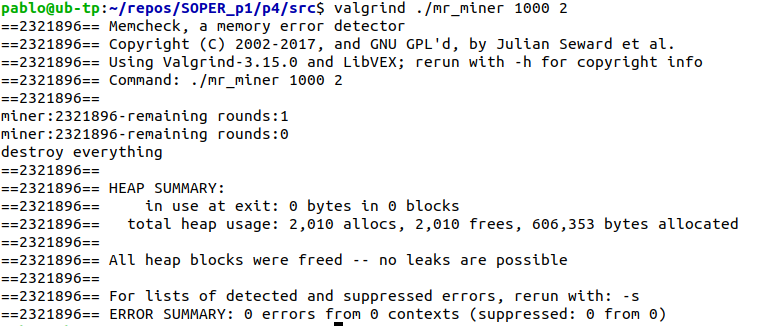
\includegraphics[scale=.41]{./pruebas/valgrind_1000_trabajadores}
        \caption{100 trabajadores con Valgrind}
    \end{figure}

    
    Dependiendo de la velocidad relativa de ejecución de los hilos (trabajadores y \textit{main}), los trabajadores pueden acabar por la llamada a \textit{pthread\_cancel} como hemos mencionado anteriormente, o por su cuenta al salir del bucle de la búsqueda de la \textbf{POW} cuando el trabajador que ha encontrado la solución cambia una variable global para indicarlo.

    
    Al finalizar las rondas de minado se imprime la cadena de vloques en un fichero para lo cual hemos usado como base la función proporcionada cambiado \textit{printf} por \textit{dprintf}. Por último,liberan todos los recursos con las respectivas funciones de \textit{free} y \textit{unlink}.

    

\addcontentsline{toc}{subsection}{Nivel 2: Comunicación con el monitor}
\subsection*{Nivel 2: Comunicación con el monitor}

    Para la comunciación con el monitor, se tiene que crear una cola de mensajes (a la que todos acceden abriéndola con su nombre). El primero en llegar la crea (sea minero o monitor), y los demás simplemente la abren.
    
    Además, el primero que llega, también crea los segmentos de memoria compartida e inicializa los campos a su respectivo valor inicial. Para evitar que dos procesos accedan a la vez en su escritura inicial, hemos tenido que usar un semáforo con nombre que impida el acceso simultáneo de dos procesos a la estructura compartida.
    Este \textit{mutex} es el único semáforo con nombre que hemos utilizado en el proyecto.

    El único minero que hay por ahora, al declararse ganador, envía por la cola de mensajes su nuevo bloque.

    El monitor, como pone en los requisitos del enunciado, no comprueba que la solución sea la correcta (con la función \emph{hash}), sino que comprueba que si tiene un bloque con ese mismo \emph{id}, el bloque recibido tenga la misma solución y objetivo. Por este motivo, y como los mineros solo mandan los bloques que se han votado como correctos, no se da nunca el caso de que el monitor reconozca un ``bloque erróneo''.

    El monitor (proceso padre) le manda a su hijo los bloques nuevos. Para mandar el número de \emph{wallets} que el hijo imprime, hemos hecho uso del campo \texttt{is\_valid} del bloque que se escribe en la tubería, que no tiene ninguna utilidad en este caso, ya que el monitor solo recibe bloques válidos y, de todas formas, el hijo del monitor nunca utiliza este campo.
    
    Debido a que tanto el padre como el hijo pueden recibir señales durante la escritura o lectura en la \textit{pipe}, hemos utilizado el siguiente algoritmo, que asegura la lectura o escritura completa de la información y el manejo de las señales en cada caso (sería similar en el caso de la escritura, cambiando \emph{read} por \emph{write}):

    \begin{lstlisting}[language=C]
do{
    size_read = read(fd[0], ((char*)block) + total_size_read, target_size - total_size_read);
    if (size_read == -1)
    {
        if(errno == EINTR && got_signal)
            handle_signal();
        else if(errno != EINTR)
            handle_read_error();
    }
    else if (size_read == 0)
        return total_size_read;
    else
        total_size_read += size_read;
} while (total_size_read != target_size);\end{lstlisting}

    En el caso del hijo, \texttt{handle\_signal()} lo que hace es poner una nueva alarma de 5 segundos e imprimir toda la cadena en su fichero.

    En el caso del padre, cuando termina la lectura y ha recibido \texttt{SIGINT}, libera todo, cerrando la tubería y termina después de que su hijo haya finalizado.

    Al terminar, si el minero o el monitor ve que ya no hay más procesos enganchados a la memoria compartida, se encarga de borrar (\emph{unlink}) los segmentos de memoria compartida, el \emph{mutex} y la cola de mensajes.

\addcontentsline{toc}{subsection}{Nivel 3: Red de mineros sin votación}
\subsection*{Nivel 3: Red de mineros sin votación}

En esta primera versión sin votación nuestro objetivo fue asegurar que los mineros empezasen las rondas a la vez, parasen de minar cuando otro minero hubiese encontrado la solución e impedir que dos mieros se declaren ganadores en una misma ronda. Los mineros que ingresan a la red deben esperar a que finalice la ronda actual, es decir, hasta que el ganador de la ronda les de paso a la siguiente ronda.

Tenemos que tener en cuenta que el ganador de una ronda se va a salir, porque esta es su última ronda (o porque ha recibido \texttt{SIGINT}), en la siguiente ronda la red pueda seguir funcionando. 
TURNSTILE:::::::::::::::::::::::::::::::::::::::::::::::::::::::::::::::::::::::::::::::::::::::: 


\addcontentsline{toc}{subsection}{Nivel 4: Red de mineros con votación}
\subsection*{Nivel 4: Red de mineros con votación}

En este nivel aseguramos además las siguientes restricciones de sincronización: los mineros perdedores no pueden empezar a votar hasta que el minero ganador haya subido la solución a memoria compartida y el minero ganador no puede empezar el recuento hasta que todos hayan votado.


\addcontentsline{toc}{section}{extra}
\section*{extra}
sigint al ganador (turnstile)

2 monitores


\end{document}

por quitar::
    
    makefile

    destroy everything
